\documentclass[aspectratio=169, table]{beamer}

\usepackage[utf8]{inputenc}
\usepackage{listings} 

\usetheme{Pradita}

\subtitle{MTI104 - IT Services}

\title{Session-01:\\\LARGE{Practices to Manage Changes\\}}
\date[Serial]{\scriptsize {PRU/SPMI/FR-BM-18/0222}}
\author[Pradita]{\small{\textbf{Alfa Yohannis}}}

\begin{document}

\frame{\titlepage}

\begin{frame}
	\frametitle{The Heart of ITIL}
	
	\begin{itemize}
		\item ITIL's core lies in operations.
		\item Value is created or lost in this phase.
		\item Customers' experiences shape their perceptions.
		\item Enhancements or developments may pause, but operations continue.
		\item Operations persist until the product’s end of support or service is active.
		\item Operations are crucial for organizational success.
	\end{itemize}
\end{frame}

% Slide 2
\begin{frame}
	\frametitle{The Role of Operations}
	
	\begin{itemize}
		\item Most action occurs during operations.
		\item Customers remember interactions during this phase.
		\item Service providers bill the most during operations.
		\item Operations are not the best place to invest heavily.
		\item The significance of operations will be explained further.
	\end{itemize}
\end{frame}

% Slide 3
\begin{frame}
	\frametitle{Operational Activities}
	
	\begin{itemize}
		\item Focus on maintaining products and services.
		\item No functional or nonfunctional modifications are made.
		\item Status quo is maintained to ensure service consistency.
		\item Operations run the longest and involve the most staff.
		\item Customer perception is formed through operational achievements.
	\end{itemize}
\end{frame}

% Slide 4
\begin{frame}
	\frametitle{Challenges in Operations}
	
	\begin{itemize}
		\item Strategies and designs may change over time.
		\item Technological innovations bring changes.
		\item Transitions and training may lead to support glitches.
		\item DevOps simplifies product and service maintenance.
	\end{itemize}
\end{frame}

% Slide 5
\begin{frame}
	\frametitle{Job Security and Trends}
	
	\begin{itemize}
		\item Operations roles offer job security.
		\item Flexibility is needed to adapt to organizational needs.
		\item DevOps professionals manage CI-CD tools and coding.
		\item Multiple skills are crucial for survival in the IT industry.
	\end{itemize}
\end{frame}

% Slide 6
\begin{frame}
	\frametitle{Practices in Operations}
	
	\begin{itemize}
		\item Monitoring and Event Management
		\item Incident Management
		\item Problem Management
		\item Important for ITIL Foundation exam.
		\item Focus on understanding these practices in depth.
	\end{itemize}
\end{frame}

% Slide 7
\begin{frame}
	\frametitle{Monitoring and Event Management}
	
	\begin{itemize}
		\item Systematically observe services and components.
		\item Record and report selected changes of state (events).
		\item Detect problems early to minimize service outages.
		\item Monitor critical Configuration Items (CIs).
	\end{itemize}
\end{frame}

% Slide 8
\begin{frame}
	\frametitle{Types of Events}
	
	\begin{itemize}
		\item Exception Events: Indicate errors, require urgent action.
		\item Warning Events: Indicate potential issues, need caution.
		\item Informational Events: Convey status changes, no urgent action required.
	\end{itemize}
\end{frame}

% Slide 9
\begin{frame}
	\frametitle{Key Activities in Monitoring}
	
	\begin{itemize}
		\item Develop monitoring strategies and designs.
		\item Define thresholds for warning and exception events.
		\item Implement monitoring tools and processes.
		\item Automation is crucial for effective monitoring.
	\end{itemize}
\end{frame}

% Slide 10
\begin{frame}
	\frametitle{Incident Management Practice}
	
	\begin{itemize}
		\item Deals with unplanned service interruptions.
		\item Affects customer satisfaction and service quality.
		\item Reacts to situations; efficiency depends on speed of resolution.
		\item Common in ITIL and critical for managing service disruptions.
	\end{itemize}
\end{frame}

\begin{frame}{Incident management life cycle}
	 \frametitle{Incident management life cycle}
\begin{center}
	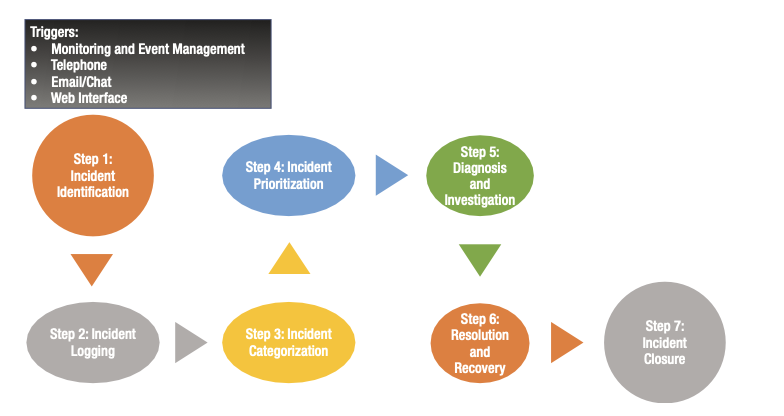
\includegraphics[width=0.8\linewidth]{images/image-01.png}
\end{center}
\end{frame}

% Slide 11
\begin{frame}
	\frametitle{Definition of an Incident}
	
	\begin{itemize}
		\item Unplanned interruption to a service or reduction in quality.
		\item Examples: Netflix buffering, email issues, hard drive failure.
		\item The goal is to restore service and minimize disruption.
	\end{itemize}
\end{frame}

\begin{frame}
	\frametitle{Introduction to Incident Management}
	\begin{itemize}
		\item An incident is a disruption to a service.
		\item Incidents are common but undesirable.
		\item Goal: Minimize incident rate and lifespan.
		\item Minimized downtime = Increased customer satisfaction.
		\item Focus: Quick resolution of incidents.
		\item Example: Netflix buffering vs. playing movie quickly.
		\item Time is essential in incident resolution.
	\end{itemize}
\end{frame}

\begin{frame}
	\frametitle{Incident Management Practice}
	\begin{itemize}
		\item Proactive vs. Reactive: Incident management is reactive.
		\item Importance: Reducing impact through quick resolution.
		\item Incidents are unavoidable; managing them is crucial.
		\item Compare to sickness: Find cure (fix) and preventive measures (immunity).
		\item Manage downtime to be minimal.
		\item Improvements like auto-reindexing to prevent issues.
	\end{itemize}
\end{frame}

\begin{frame}
	\frametitle{Incident Management Practices}
	\begin{itemize}
		\item Log all incidents, including internal staff findings.
		\item Implement self-help tools for hands-free operations.
		\item Have a capable service desk as the first contact.
		\item Establish a functional escalation matrix.
		\item Maintain a matrix of responsible teams for incidents.
		\item Involve all stakeholders in incident resolution.
		\item Build specialized teams for critical incidents.
	\end{itemize}
\end{frame}

\begin{frame}
	\frametitle{Good Practices in Incident Management}
	\begin{itemize}
		\item Use swarming techniques for initial resolution stages.
		\item Address service continuity through disaster recovery plans.
		\item Record all updates on an incident register.
		\item Service continuity management ensures service endures during disasters.
		\item Techniques: Data replication, disaster recovery, resilience building.
	\end{itemize}
\end{frame}

\begin{frame}
	\frametitle{Incident Management Life Cycle}
	\begin{itemize}
		\item Various incidents need standardized management.
		\item Life cycle steps can vary by implementation.
		\item Example steps:
		\begin{enumerate}
			\item Incident Identification
			\item Incident Logging
			\item Incident Categorization
			\item Incident Prioritization and Investigation
			\item Diagnosis
			\item Resolution
			\item Incident Closure
		\end{enumerate}
	\end{itemize}
\end{frame}

\begin{frame}
	\frametitle{Incident Identification}
	\begin{itemize}
		\item Incidents must be identified via triggers.
		\item Common triggers:
		\begin{itemize}
			\item Monitoring and Event Management
			\item Telephone
			\item Email/Chat
			\item Web Interface
		\end{itemize}
		\item Importance of identifying and managing triggers.
	\end{itemize}
\end{frame}

\begin{frame}
	\frametitle{Incident Logging}
	\begin{itemize}
		\item Log all identified incidents with timestamps.
		\item Use ITSM tools like ServiceNow, BMC Remedy.
		\item Common fields on incident tickets:
		\begin{itemize}
			\item Incident number, End user name, Time of logging
			\item Impact, Urgency, Priority, Category
			\item Incident summary, Assigned resolver group
		\end{itemize}
	\end{itemize}
\end{frame}

\begin{frame}
	\frametitle{Incident Categorization}
	\begin{itemize}
		\item Categorize incidents into appropriate buckets.
		\item Correct categorization is crucial for effective resolution.
		\item Example: Network issue vs. application issue.
		\item Autologged and user-raised incidents may require careful categorization.
	\end{itemize}
\end{frame}

\begin{frame}
	\frametitle{Incident Prioritization}
	\begin{itemize}
		\item Prioritization based on impact and urgency.
		\item Examples:
		\begin{itemize}
			\item Major impact and urgent = High priority
			\item Minor impact and non-urgent = Low priority
		\end{itemize}
		\item Priority determined by a matrix.
		\item Response SLA and Resolution SLA are defined.
	\end{itemize}
\end{frame}

\begin{frame}{Incident priority matrix}
	 \frametitle{ Incident priority matrix}
\begin{center}
	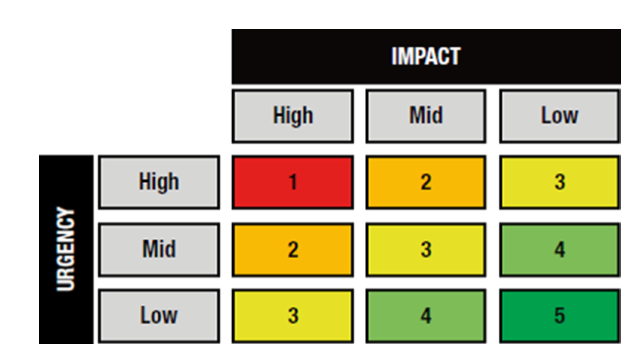
\includegraphics[width=0.8\linewidth]{images/image-02.png}
\end{center}
\end{frame}

\begin{frame}
	\frametitle{Incident Priorities and SLAs}
	\begin{itemize}
		\item Incident priorities may change during the life cycle.
		\item Response SLA: Time to acknowledge the incident.
		\item Resolution SLA: Time to resolve the incident.
		\item Example: P1 priority with 15-minute response and 2-hour resolution.
		\item SLAs vary by customer requirements and incident priority.
	\end{itemize}
\end{frame}

\begin{frame}{Incident management SLAs}
	 \frametitle{ Incident management SLAs}
\begin{center}
	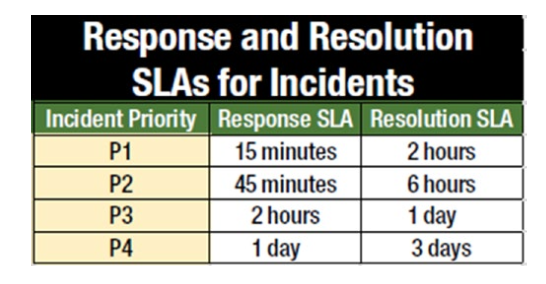
\includegraphics[width=0.8\linewidth]{images/image-03.png}
\end{center}
\end{frame}

\begin{frame}
	\frametitle{Step 5: Diagnosis and Investigation}
	\begin{itemize}
		\item Initial diagnosis by understanding symptoms
		\item Identify what's not working
		\item Basic troubleshooting steps
		\item Analogous to a doctor asking about symptoms
		\item Key substep providing data for further investigation
		\item Service desk may escalate to level 2 (L2) support
		\item L2 groups: server, network, storage, or software experts
	\end{itemize}
\end{frame}

% Slide 2
\begin{frame}
	\frametitle{Step 5: Diagnosis and Investigation (cont.)}
	\begin{itemize}
		\item Resolver group uses available information
		\item May call user for more details
		\item Incorrect questioning may lead to starting over
		\item Investigation involves:
		\begin{itemize}
			\item User expectations
			\item What went wrong
			\item Sequence of steps
			\item Impact and scope
			\item Recent changes
			\item Similar incidents or KEDB articles
		\end{itemize}
	\end{itemize}
\end{frame}

% Slide 3
\begin{frame}
	\frametitle{Step 6: Resolution and Recovery}
	\begin{itemize}
		\item Apply resolutions based on investigation
		\item Troubleshoot at appropriate level (server or network)
		\item Success depends on correct investigation path
		\item Tests and recovery period for widespread incidents
		\item Major incidents may remain open for observation
		\item Daily/hourly meetings with stakeholders
	\end{itemize}
\end{frame}

% Slide 4
\begin{frame}
	\frametitle{Step 7: Incident Closure}
	\begin{itemize}
		\item Confirm with user before closing ticket
		\item Service desk handles confirmation
		\item Alternative: Incident remains resolved for 3 days
		\item Email to user for confirmation
		\item Autoclosure if no response
		\item User satisfaction survey post-closure
	\end{itemize}
\end{frame}

% Slide 5
\begin{frame}
	\frametitle{Major Incident Management}
	\begin{itemize}
		\item Major incidents: High impact and potential damage
		\item Separate process with stringent timelines
		\item Major incident managers handle these incidents
		\item High pressure and responsibility
		\item Separate team and specialized skill sets
		\item Communication and updates to all stakeholders
	\end{itemize}
\end{frame}

% Slide 6
\begin{frame}
	\frametitle{Engagement with Service Value Chain}
	\begin{itemize}
		\item Plan: Low involvement in incident management
		\item Design and Transition: Medium involvement
		\item Obtain/Build: Medium involvement
		\item Engage: High involvement
		\item Deliver and Support: High involvement
		\item Improve: Medium involvement
	\end{itemize}
\end{frame}

% Slide 7
\begin{frame}
	\frametitle{Problem Management Practice}
	\begin{itemize}
		\item Incident management: Immediate relief
		\item Problem management: Long-term prevention
		\item Focus on root causes of incidents
		\item Problem management as the "CSI" of IT
		\item Example: Application crash and resolution
		\item Prevention through problem management
	\end{itemize}
\end{frame}

% Slide 8
\begin{frame}
	\frametitle{ITIL Definition of Problem}
	\begin{itemize}
		\item Cause or potential cause of incidents
		\item Unresolved incidents until root cause is known
		\item Avoiding guesswork in solutions
		\item Example: Doctor prescribing without diagnosis
		\item Problem management seeks root causes
	\end{itemize}
\end{frame}

% Slide 9
\begin{frame}
	\frametitle{Incidents vs. Problems}
	\begin{itemize}
		\item Incidents: Loss or degradation of services
		\item Problems: Root causes of incidents
		\item Problems arise when root cause is unknown
		\item Example: Software application crash
		\item Problem management for permanent solutions
	\end{itemize}
\end{frame}

% Slide 10
\begin{frame}
	\frametitle{Other Key Terminologies in Problem Management}
	\begin{itemize}
		\item Root Cause: Fundamental reason for an incident
		\item Root-Cause Analysis (RCA): Techniques to find root cause
		\item Known Error: Analyzed problem with no permanent fix
		\item Known Error Database (KEDB): Repository of known errors
		\item Workaround: Temporary fix for incidents
		\item Permanent Solution: Long-term resolution of root cause
	\end{itemize}
\end{frame}

% Slide 11
\begin{frame}
	\frametitle{Problem Management Phases}
	\begin{itemize}
		\item Problem Identification: Finding the problem
		\item Problem Control: Analyzing and prioritizing problems
		\item Error Control: Implementing permanent solutions
		\item Techniques: Brainstorming, Five-Why, Ishikawa Diagram
	\end{itemize}
\end{frame}

\begin{frame}{Problem management phases}
	 \frametitle{ Problem management phases}
\begin{center}
	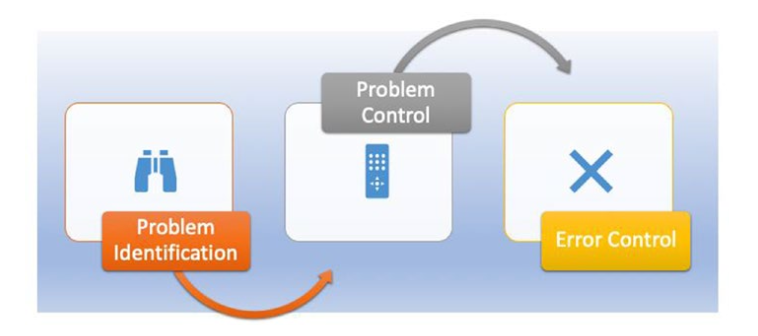
\includegraphics[width=0.8\linewidth]{images/image-04.png}
\end{center}
\end{frame}

\begin{frame}
	\frametitle{Multiple Choice Question}
	
	Which of the following is the correct event definition?
	\begin{enumerate}[A.]
		\item Any change of state that is significant for a service or product or related CI
		\item Any change of state that triggers changes to the other operational processes
		\item Any change of state for CIs that correlates risks and issues to the service and service management processes
		\item Any change of state that has significance for the management of a service or other CI
	\end{enumerate}
	
\end{frame}


\end{document}
